%% Beginning of file 'PASPsample631.tex'

%% using aastex version 6.3.1
\documentclass[twocolumn]{aastex631}
\newcommand{\vdag}{(v)^\dagger}
\newcommand\aastex{AAS\TeX}
\newcommand\latex{La\TeX}


\begin{document}

\title{Properties of Bulge and Disk Particles in the Milky Way and M31 Merger Remnant}

\author{Ellen Jesina}
\affiliation{The University of Arizona\\
Tucson, AZ 85719}

\section{Introduction} \label{sec:intro}
%Define proposed topic & how it pertains to Galaxy Evolution. Describe the general area of galaxy structure/dynamics and/or evolution
My topic of interest involves looking into how the bulge and the disk compare when analyzing their contributions to density profiles, shapes, velocity dispersions, and angular momenta of the merger remnant. This merger remnant specifically refers to that which will form when the Milky Way Galaxy and M31, commonly known as the Andromeda Galaxy, eventually collide. When galaxies collide, it is important to focus on the bulge's and the disk's evolution to understand the overall evolution of these galaxies, particularly if we want to understand what particles continue rotating, if any. 


%State why this topic matters to our understanding of galaxy evolution
This topic if important to understanding how galaxies evolve as they merge overall. We can discover if one galaxy becomes more dominant, for example, or which particles are more likely to be dynamically changed through a galactic merger. Furthermore, studying our own galaxy's evolution, in particular, can offer us insight into its fate and enable us to better understand its interactions with other galaxies. This can even include how this can impact our own Solar System, since it is likely that this event will occur within the Sun's lifetime (\cite{Cox_2008}). In our case, we are looking into how the remnant of this merger behaves. This remnant, or what is left and formed after the two galaxies merge, is important to understand how different particles behave and evolve so we can understand galactic dynamics more thoroughly. Furthermore, galaxy mergers are important to study in order to understand how not only our own galaxy will evolve, but also so that we can better understand the evolution of galaxies we can observe. The analysis of one or the other can be easily applied to both areas so that we understand galactic dynamics and how the universe has formed as a whole. 

%Overview our current understanding of the topic in galaxy evolution, very broadly
It is commonly understood that the Milky Way and Andromeda will eventually merge due to their gravitational attraction. This is expected to happen in the next 5 Gyr (\cite{Cox_2008}) and can be seen in Figure \ref{Figure 1}. Galaxy mergers are dependent not only on the size, or mass, of the galaxies merging (\cite{10.1111/j.1365-2966.2010.16268.x}), but also the amount of angular momentum (\cite{2008ApJS..175..356H}). It can even depend on the baryonic mass in particular (\cite{10.1111/j.1365-2966.2010.16268.x}), though this is more variable when it comes to smaller galaxy mergers as compared to large galaxies like the Milky Way and Andromeda. Recent research has studied the timescales of this merger (\cite{Cox_2008}), though the explicit dynamics of how our own galaxy will evolve is limited in literature. Much of our understanding comes from how we observe other galaxies merge, visually and dynamically. 

\begin{figure}
    \centering
    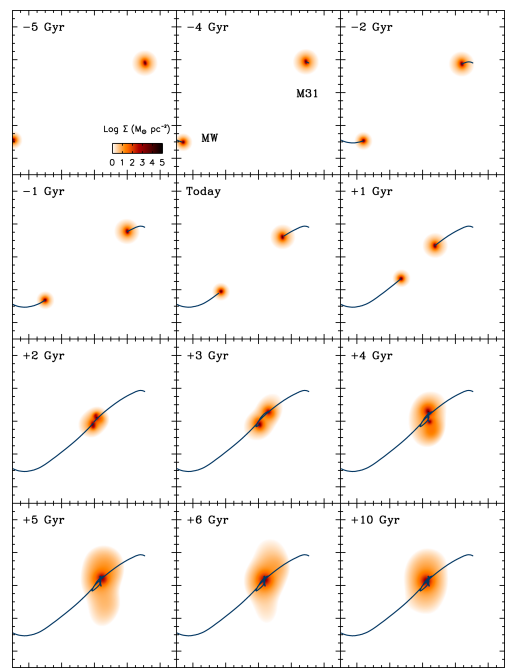
\includegraphics[width = 0.5\textwidth]{Figure 2 from Cox (2008).png}
    \label{Figure 1}
    \caption{Taken from \cite{Cox_2008} Projected stellar density throughout the merger of Andromeda (starting in the upper right) and the Milky Way. It is projected to take approximately 5 Gyr from today. }
\end{figure}

%What are the open questions pertaining to this topic?
Open questions relating to this topic typically revolve around the desire to better understand how the merger remnant would compare to other galactic merger remnants that we can observe. This particularly pertains to the shape of the galaxy remnant and its luminosity. The shape is expected to be elliptical (\cite{Cox_2008}) and the luminosity is expected to be moderate from recent assumptions, but further modeling can confirm if this is the future fate of our galaxy. There are also several questions about how this merger event and its remnant could have an impact on our own Solar System. For example, there is the likelihood of the Sun being absorbed by Andromeda during a close pass-by (\cite{Cox_2008}), and the possibility of part of the merger being visible to future humans. These questions could be constrained through future modeling, but they may also have to wait until our galaxy advances further in its own evolution. 

Further unanswered questions pertain to what the angular momentum is of a galaxy merger remnant. This question was called ambiguous by \cite{2008ApJS..175..356H}, since it somewhat depends on circular and orbital frequencies of the galaxies merging. There are also only certain angular momenta that are believed to enable galaxies to merge (\cite{2008ApJS..175..356H}), otherwise there may be not enough momentum to merge, resulting in very gradual tidal accretion. Looking into the angular momentum of the resulting merger can offer insight into the general momentum required to merge and can explain even black hole dynamics when merging, as initially investigated by \cite{2008ApJS..175..356H}. 

%must cite at least 3 papers, including at least one image

\section{The Proposal} \label{sec:style}

\subsection{Questions}
%what questions will I be addressing in the simulation
The main question I will be answering is: How do the bulge and disk of the galaxy remnant contribute to various aspects of the merger remnant? These various aspects include the density profile, the overall shape, the velocity dispersion, and the overall angular momentum. These aspects will enable a better understanding of the overall evolution, and it can also offer insight into what parts of the galactic remnant are rotating. Understanding rotation requires an understanding of the aforementioned angular momentum, as we need to determine if it is conserved through such a large event like a galactic merger. We must also determine if there are rotating particles in the remnant so that we can understand the merger's evolutionary history and investigate how initial and final angular momentum affect the merger and its remnants. 

\subsection{Methods}
%How will I approach the specific question using simulation data? Define all relevant equations and terms and outline all the code I will be using. Also must include at least one figure
In order to understand how the bulge and disk influence the density profile, shape, velocity, and angular momentum of the galaxy remnant, we can utilize simulations through coding. To begin, we must find the snapshot point in our text files where we see the Milky Way and Andromeda merge. Once we have this point, we can adapt our code to be at this snapshot and beyond as this will now be part of the merger remnant, allowing us to use the results to answer our questions. These snapshots range from 0-801, and we anticipate seeing similarities in the bulge and disk of M31 and the Milky Way past the merger point, providing us with enough information to have redundancy. 

Once we have this snapshot, we will use this point to calculate the velocity profiles and dispersions of the two galaxies. At this point, since they have merged, these should match. This will be used to then compare to the velocity profile of a spiral structure. We can also use the snapshot to determine the mass profile of the new remnant, which we have previously analyzed in Labs (such as lab 7) and in homeworks (such as in homework 5). This mass profile, in turn, can be used to determine the density profile by plotting the mass profile against the volume as a function of the radius, or distance from the new determined center of mass. This will be done for both the disk and the bulge. 

Next, we will use the velocity and the mass as a function of radius specifically around the center of mass to determine angular momentum. Since angular momentum is dependent on the mass, angular velocity, and radius, this can be easily determined from the aforementioned code we have done in class and in homeworks. Determining this angular momentum will allow us to determine if the bulge and/or disk are rotating around the new center of mass. Furthermore, considering angular momentum must be conserved and our mass and radius are increasing significantly, it would make sense that rotational velocity decreases to be essentially zero. 
In turn, this can further confirm our findings about the shape of the galaxy and confirm the hypotheses mentioned in the following section.
A summary of this outline can be seen clearly in \ref{Figure 2}


\begin{figure}
    \centering
    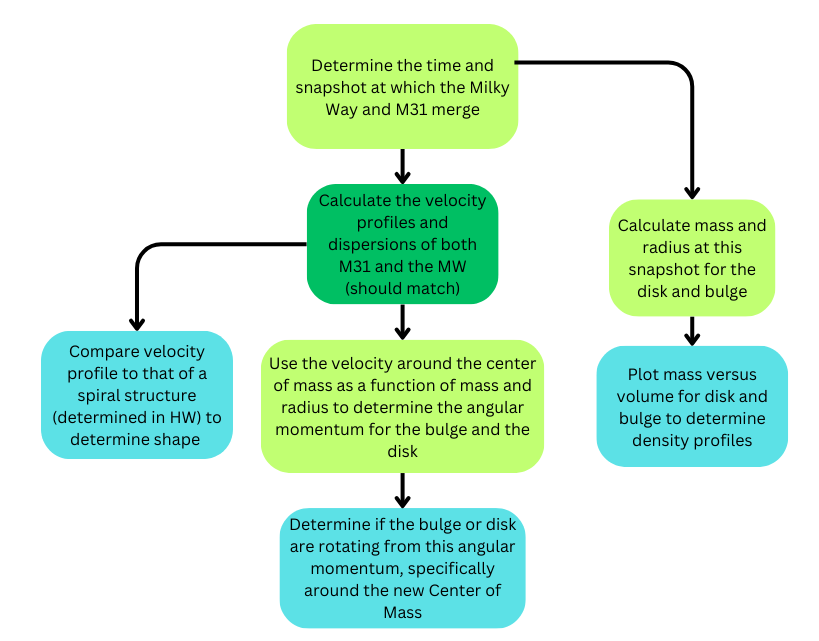
\includegraphics[width = 0.45\textwidth]{400B Flow chart.png}
    \label{Figure 2}
    \caption{Flow Chart showing anticipated stages of this research. The light green shows the information the code will enable us to find. The dark green shows the information we receive from the code that can be used for determining answers to our other questions as well as provide an answer in itself. Finally, the light blue shows the resulting information we anticipate to be obtainable within this research.}
\end{figure}

\subsection{Hypothesis}
%What is my hypothesis for what I will find, and why do I think this will occur?
Based on the preceding information, my hypothesis is that we will find a merger remnant that has an elliptical shape. This implies that there will be relatively low angular momentum as well as a more uniform density distribution than before the merger. Furthermore, since it will likely result in an elliptical galaxy, there will not be a component that is noticeably rotating. I further anticipate the velocity dispersion to be somewhat even and somewhat low as elliptical galaxies do not show significant rotation as compared to spiral galaxies. I believe this is the likely scenario considering previous work done that shows a merger is imminent, and information from these papers and from what we have learned and done in classes to explain galactic mergers. 


%\software{astropy \citep{2013A&A...558A..33A,2018AJ....156..123A},  
          %Cloudy \citep{2013RMxAA..49..137F}, 
          %Source Extractor \citep{1996A&AS..117..393B}
          %}

%\section{Bibliography}
%\bibliography{Research Project}{}
\bibliography{bibliography}


\end{document}